\documentclass[tikz]{standalone}

\usetikzlibrary{calc,positioning,shapes,positioning,intersections,quotes,decorations.markings}
\usepackage{amsfonts,amsmath,amsthm,amssymb,mathtools,stmaryrd,mathrsfs}

\begin{document}
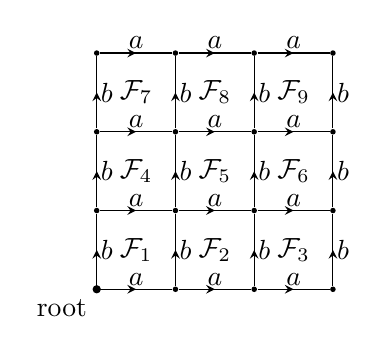
\begin{tikzpicture}[>=stealth,decoration={
				markings,
				mark=at position 0.5 with {\arrow{>}}}
	]

	\node[circle,fill=black,inner sep=0pt,minimum size=3pt] (root) at (0,0){} node[below left]{root};

	\foreach \x in {0,1,2,3} {
			\foreach \y in {0,1,2,3} {
					\node[circle,fill=black,inner sep=0pt,minimum size=2pt] (n\x_\y) at (\x,\y) {};
				}
		}

	\foreach \x [count=\xx from 1] in {0,1,2} {
			\foreach \y in {0,1,2,3} {
					\draw[postaction={decorate}] (n\x_\y) --node[above=-2pt]{$a$} (n\xx_\y);}
		}

	\foreach \x in {0,1,2,3} {
			\foreach \y [count=\yy from 1] in {0,1,2} {
					\draw[postaction={decorate}] (n\x_\y) --node[right=-2pt]{$b$} (n\x_\yy);}
		}

  \node (f1) at (0.5,0.5) {$\mathcal F_1$};
  \node (f2) at (1.5,0.5) {$\mathcal F_2$};
  \node (f3) at (2.5,0.5) {$\mathcal F_3$};

  \node (f4) at (0.5,1.5) {$\mathcal F_4$};
  \node (f5) at (1.5,1.5) {$\mathcal F_5$};
  \node (f6) at (2.5,1.5) {$\mathcal F_6$};

  \node (f7) at (0.5,2.5) {$\mathcal F_7$};
  \node (f8) at (1.5,2.5) {$\mathcal F_8$};
  \node (f9) at (2.5,2.5) {$\mathcal F_9$};

\end{tikzpicture}
\end{document}
